\documentclass[10pt, a4paper]{article}
\usepackage{a4wide}
\usepackage[T1]{fontenc}
\usepackage[utf8]{inputenc}
\usepackage{float, afterpage, rotating, graphicx}
\usepackage{epstopdf}
\usepackage{longtable, booktabs, tabularx}
\usepackage{fancyvrb, moreverb, relsize}
\usepackage{eurosym, calc, chngcntr}
\usepackage{amsmath, amssymb, amsfonts, amsthm, bm}
\usepackage{caption}
\usepackage{mdwlist}
\usepackage{xfrac}
\usepackage{setspace}
\usepackage{xcolor}
\usepackage[super]{nth}
\usepackage[labelfont=bf]{caption}
% \usepackage{pdf14} % Enable for Manuscriptcentral -- can't handle pdf 1.5
% \usepackage{endfloat} % Enable to move tables / figures to the end. Useful for some submissions.
% Sublabeling of figures
\usepackage{subfloat}

\usepackage[
    natbib=true,
    bibencoding=inputenc,
    bibstyle=authoryear-ibid,
    citestyle=authoryear-comp,
    maxcitenames=3,
    maxbibnames=10,
    useprefix=false,
    sortcites=true,
    backend=bibtex
]{biblatex}
\AtBeginDocument{\toggletrue{blx@useprefix}}
\AtBeginBibliography{\togglefalse{blx@useprefix}}
\setlength{\bibitemsep}{1.5ex}
\addbibresource{refs.bib}

\usepackage[unicode=true]{hyperref}
\hypersetup{
    colorlinks=true,
    linkcolor=black,
    anchorcolor=black,
    citecolor=black,
    filecolor=black,
    menucolor=black,
    runcolor=black,
    urlcolor=black
}


\widowpenalty=10000
\clubpenalty=10000

\setlength{\parskip}{1ex}
\setlength{\parindent}{0ex}
\setstretch{1.5}

% reduce size of section headings
\usepackage{titlesec}

\titleformat{\section}
{\normalfont\fontsize{11}{15}\bfseries}{\thesection}{1em}{}
\titlespacing\section{0pt}{10pt plus 4pt minus 2pt}{0pt plus 2pt minus 2pt}
\titlespacing\subsection{0pt}{8pt plus 1pt minus 4pt}{0pt plus 2pt minus 2pt}
\titlespacing\subsubsection{0pt}{8pt plus 1pt minus 4pt}{0pt plus 2pt minus 2pt}

\begin{document}

\title{The Swiss case: Reactions of the real economy to the discontinuation of the exchange rate floor in 2015. A synthetic control approach
\thanks{Martin Dohmen: University of Bonn, Address. \href{mailto:x@y.z} {\nolinkurl{s3madohm[at]uni-bonn[dot]de}}}
% subtitle: 
% \\[1ex] 
% \large Subtitle here
}

\author{Martin Dohmen
% \\[1ex]
% Additional authors here
}

\date{
{\bf Preliminary -- please do not quote} 
\\[1ex] 
\today
}

\maketitle



\clearpage


\section{The Synthetic Control Method} % (fold)
\label{sec:method} 

In this section I want to give a short description of the synthetic control method. It follows mainly \citet{Abadie2010}. For details please refer to this paper and to \citet{Abadie2014} and \citet{Becker2018}.

The synthetic control method is a data-driven approach to construct a suitable control unit in comparative case studies. The idea is that a combination of control units will often provide a better comparison for the treated unit than a single control unit alone. Therefore, the synthetic control is constructed as a weighted average of so called donors, a sample of suitable control units, with non-negative weights that sum to one. These weights, collected in a vector $W$, are calculated by minimizing the difference of selected predictor variables between the treated unit and the synthetic control. The predictor variables can be linear combinations of the outcome variable prior to treatment as well as other covariates with explanatory power for the outcome of interest, which need to be measured prior to or unaffected by the treatment. In the optimization the predictors are weighted by a predictor weighting matrix $V$, which is chosen to result in optimal weights $W$ that yield the lowest possible RMSPE between the outcome of the treated unit and the synthetic control prior to treatment. This structure leads to a nested optimization problem. In the inner optimization the optimal donor weights $W$ are determined, which construct the synthetic control unit. These optimization depends on the predictor weights $V$, which are determined in the outer optimization to guarantee the best possible pre-treatment fit. The resulting optimal weights define the synthetic control unit. The treatment effect consists of the difference in the outcome variable after treatment between the treated unit and the synthetic control.



\section{Implementation} % (fold)
\label{sec:implementation} 

The structure of the synthetic control method described above poses some challenges to the implementation. The problem is that the nested optimization is not only computational intensive and therefore slow with larger data sets, but it might also be quite unstable and unreliable with numerical optimizers. The reason for that is that the objective function of the outer optimization contains a minimization problem, which results in a noisy function that might be ill behaved and can fool the outer optimizer. \citet{Becker2018} provide an algorithm that tries to reduce these problems. It starts with detecting important special cases that are easy to compute and then tries to reduce the dimension of the nested optimization problem.

The basis of Becker and Klößner's argumentation consists of some theory concerning the optimization problems that have to be solved for applying the synthetic control method. They start with separating the donor pool in sunny and shady donors. A shady donor is a control unit, whose difference in predictor values to the treated unit multiplied by $\alpha$ with $0<\alpha<1$ lies inside the convex hull of the differences of all donor units. They show that if a donor is shady, it will not be part of an optimal synthetic control unit. Furthermore, they give simple solutions in cases with no sunny donors, which means exact fit is possible, or only one sunny donor, which will then be the unique donor with positive weight. If none of these special cases occur, the algorithm tests whether the unrestricted outer optimum is feasible. This means it searches for predictor weights $V$ which result in donor weights $W$ that constitute the global minimum of the outer optimization problem. Only if finding such predictor weights is not possible, the nested optimization is performed. In order to do this, the dimension of the problem is reduced by excluding all shady donors. A detailed description of the algorithm can be found in \citet{Becker2018} and Figure 2 in their paper illustrate it's structure in a simple way.

I implement this algorithm in a python program. For optimizers and solvers to the linear programs I rely on the open source library scipy, which is used for scientific computation. During the implementation I had to make some design choices and I deviate from the algorithm at one place. This deviation occurs in the special case when no sunny donors are found, so that exact fit is possible. As the optimizers in scipy can not deal with situations with more equality constraints than independent variables, I choose to take a short cut there. In this case my program will only perform the inner minimization and print a warning. This will result in weights that lead to exact fit of the synthetic control regarding the predictors, but, if multiple such weights exist, it might choose a suboptimal solution regarding the outer optimization. In my opinion this is not major concern as this special case is very rare. The program will return a warning informing the user and suggesting to increase the number of predictor variables. The more predictors, the less likely it will become that exact fit is possible and that there are no sunny donors. In an extreme case all outcome variables defining the outer optimization could be chosen as predictors, which would render the problem unimportant as inner and outer optimization would coincide.

For the nested optimization I followed the algorithm closely. However, the suggested method for the inner optimization is not implemented in scipy. Instead I relied on sequential least squares programming to solve the inner minimization, as it can handle equality constraints and bounds for independent variables. This leads to the problem that the inner optimization is slower and much more noisy than in the implementation by Becker and Klößner. For the outer optimization I relied on the method L-BFGS-B, as routines using this algorithm performed quite well in their tests. Nevertheless, this combination of optimizers still lead to a quite unstable nested optimization. In some, more complex cases the outer optimizer is not capable of handling the noisy and sometimes ill behaved inner objective function. This did not change when I used other outer optimizers in scipy capable of box constrained minimization.  





\clearpage


%\counterwithin{table}{section}
% APPENDIX
\section{Appendix} % (fold)
\label{sec:appendix} 

The programming code is available on request. The program is based on the template for economic programming by \citet{GaudeckerEconProjectTemplates}.

 

\subsection{Tables} % (fold)
\label{sec:tables} 

% TABLES FOR WEIGHTS OF GDPPC SPECIFICATIONS
\begin{table}[H]
	\renewcommand{\thetable}{\arabic{table}a}
	\caption{Weights specification 1: GDP per capita, baseline}
	\label{tab:weights baseline}
	\centering
	\begin{tabular}{c|c|c}
\textbf{Country}&\textbf{Sunny Donor}&\textbf{Weight}\\
\hline 
Australia & Yes & 0.3862 \\ 
Austria & Yes & 0.1021 \\ 
Belgium & Yes & 0.0320 \\ 
Canada & No & 0.0000 \\ 
Czech Republic & No & 0.0000 \\ 
Denmark & No & 0.0000 \\ 
Finland & Yes & 0.0000 \\ 
Hungary & No & 0.0000 \\ 
Iceland & Yes & 0.0000 \\ 
Luxembourg & Yes & 0.1843 \\ 
Netherlands & No & 0.0000 \\ 
New Zealand & Yes & 0.0000 \\ 
Norway & Yes & 0.1366 \\ 
Sweden & No & 0.0000 \\ 
United Kingdom & No & 0.0000 \\ 
United States & Yes & 0.1589 \\ 
\end{tabular}
\end{table}

\begin{table}[H]
	\addtocounter{table}{-1}
	\renewcommand{\thetable}{\arabic{table}b}
	\caption{Weights specification 2: GDP per capita, all year averages as predictors}
	\label{tab:weights all years}
	\centering
	\begin{tabular}{c|c|c}
\textbf{Country}&\textbf{Sunny Donor}&\textbf{Weight}\\
\hline 
Australia & Yes & 0.7012 \\ 
Austria & Yes & 0.0000 \\ 
Belgium & Yes & 0.0000 \\ 
Canada & Yes & 0.0000 \\ 
Czech Republic & Yes & 0.0000 \\ 
Denmark & Yes & 0.0000 \\ 
Finland & Yes & 0.0000 \\ 
Hungary & Yes & 0.0000 \\ 
Iceland & Yes & 0.0000 \\ 
Luxembourg & Yes & 0.2421 \\ 
Netherlands & Yes & 0.0000 \\ 
New Zealand & Yes & 0.0000 \\ 
Norway & Yes & 0.0567 \\ 
Sweden & Yes & 0.0000 \\ 
United Kingdom & Yes & 0.0000 \\ 
United States & Yes & 0.0000 \\ 
\end{tabular}
\end{table}

\begin{table}[H]
	\addtocounter{table}{-1}
	\renewcommand{\thetable}{\arabic{table}c}
	\caption{Weights specification 3: GDP per capita, with covariates as predictors}
	\label{tab:weights with covariates}
	\centering
	\begin{tabular}{c|c|c}
\textbf{Country}&\textbf{Sunny Donor}&\textbf{Weight}\\
\hline 
Australia & No & 0.0000 \\ 
Austria & No & 0.0000 \\ 
Belgium & Yes & 0.0000 \\ 
Canada & Yes & 0.0460 \\ 
Czech Republic & Yes & 0.2050 \\ 
Denmark & No & 0.0000 \\ 
Finland & No & 0.0000 \\ 
Hungary & Yes & 0.0000 \\ 
Iceland & No & 0.0000 \\ 
Luxembourg & Yes & 0.1856 \\ 
Netherlands & No & 0.0000 \\ 
New Zealand & Yes & 0.0000 \\ 
Norway & Yes & 0.1818 \\ 
Sweden & Yes & 0.0000 \\ 
United Kingdom & Yes & 0.0000 \\ 
United States & Yes & 0.3818 \\ 
\end{tabular}
\end{table}


% TABLES FOR PREDICTORS OF GDPPC SPECIFICATIONS
\begin{table}[H]
	\renewcommand{\thetable}{\arabic{table}a}
	\caption{Predictors specification 1: GDP per capita, baseline}
	\label{tab:predictors baseline}
	\centering
	\begin{tabular}{c|c|c}
predictor&\textbf{treated country}&\textbf{synthetic control}\\
\hline 
GDPPC 2008 & 53743.67 & 53784.62\\
GDPPC 2010 & 52857.98 & 52799.27\\
GDPPC 2012 & 53432.64 & 53330.78\\
GDPPC 2013 & 53818.96 & 53600.88\\
GDPPC 2014 & 54465.20 & 54518.70\\
\hline
\end{tabular}
\end{table}

\begin{table}[H]
	\addtocounter{table}{-1}
	\renewcommand{\thetable}{\arabic{table}b}
	\caption{Predictors specification 2: GDP per capita, all year averages as predictors}
	\label{tab:predictors all years}
	\centering
	\begin{tabular}{c|c|c}
predictor&\textbf{treated country}&\textbf{synthetic control}\\
\hline 
GDPPC 2007 & 53268.45 & 53954.39\\
GDPPC 2008 & 53743.67 & 53433.02\\
GDPPC 2009 & 51916.30 & 51985.97\\
GDPPC 2010 & 52857.98 & 52785.30\\
GDPPC 2011 & 53487.37 & 53184.26\\
GDPPC 2012 & 53432.64 & 53277.67\\
GDPPC 2013 & 53818.96 & 53610.47\\
GDPPC 2014 & 54465.20 & 54624.97\\
\hline
\end{tabular}
\end{table}

\begin{table}[H]
	\addtocounter{table}{-1}
	\renewcommand{\thetable}{\arabic{table}c}
	\caption{Predictors specification 3: GDP per capita, with covariates as predictors}
	\label{tab:predictors with covariates}
	\centering
	\begin{tabular}{c|c|c}
predictor&\textbf{treated country}&\textbf{synthetic control}\\
\hline 
GDPPC 2012-2014 & 53905.60 & 53218.99\\
Trade Openness & 124.11 & 124.29\\
Industry Share & 26.33 & 26.33\\
Inflation Rate & -0.31 & 1.68\\
Schooling & 84.18 & 84.16\\
\hline
\end{tabular}
\end{table}

% TABLE WEIGHTS FOR CA SPECIFICATION

\begin{table}[H]
	\renewcommand{\thetable}{\arabic{table}}
	\caption{Weights for current account specification}
	\label{tab:weights ca}
	\centering
	\begin{tabular}{c|c|c}
\textbf{Country}&\textbf{Sunny Donor}&\textbf{Weight}\\
\hline 
Australia & No & 0.0000 \\ 
Austria & No & 0.0000 \\ 
Belgium & Yes & 0.0000 \\ 
Czech Republic & Yes & 0.0000 \\ 
Denmark & Yes & 0.1841 \\ 
Finland & No & 0.0000 \\ 
Hungary & No & 0.0000 \\ 
Iceland & No & 0.0000 \\ 
Luxembourg & Yes & 0.0126 \\ 
Netherlands & Yes & 0.5369 \\ 
New Zealand & Yes & 0.0000 \\ 
Norway & Yes & 0.2664 \\ 
Sweden & Yes & 0.0000 \\ 
United Kingdom & No & 0.0000 \\ 
United States & Yes & 0.0000 \\ 
\end{tabular}
\end{table}

% TABLE PREDICTORS FOR CA SPECIFICATION

\begin{table}[H]
	\renewcommand{\thetable}{\arabic{table}}
	\caption{Predictors for current account specification}
	\label{tab:predictors ca}
	\centering
	\begin{tabular}{c|c|c}
predictor&\textbf{treated country}&\textbf{synthetic control}\\
\hline 
Current Account 2012-2014 & 10.04 & 9.75\\
Trade Openness & 124.11 & 124.24\\
Industry Share & 26.33 & 26.44\\
Inflation Rate & -0.31 & 1.75\\
Schooling & 84.18 & 72.45\\
\hline
\end{tabular}
\end{table}

% WEIGHTS PLACEBO SPECIFICATIONS

\begin{table}[H]
	\renewcommand{\thetable}{\arabic{table}a}
	\caption{Weights for time placebo specification}
	\label{tab:weights time placebo}
	\centering
	\begin{tabular}{c|c|c}
\textbf{Country}&\textbf{Sunny Donor}&\textbf{Weight}\\
\hline 
Australia & Yes & 0.0000 \\ 
Austria & Yes & 0.0000 \\ 
Belgium & Yes & 0.0000 \\ 
Canada & No & 0.0000 \\ 
Czech Republic & Yes & 0.0000 \\ 
Denmark & Yes & 0.5258 \\ 
Finland & No & 0.0000 \\ 
Hungary & Yes & 0.0000 \\ 
Iceland & Yes & 0.0000 \\ 
Luxembourg & Yes & 0.0000 \\ 
Netherlands & Yes & 0.0000 \\ 
New Zealand & No & 0.0000 \\ 
Norway & Yes & 0.4742 \\ 
Sweden & No & 0.0000 \\ 
United Kingdom & Yes & 0.0000 \\ 
United States & Yes & 0.0000 \\ 
\end{tabular}
\end{table}

\begin{table}[H]
	\addtocounter{table}{-1}
	\renewcommand{\thetable}{\arabic{table}b}
	\caption{Weights for country placebo specification}
	\label{tab:weights country placebo}
	\centering
	\begin{tabular}{c|c|c}
\textbf{Country}&\textbf{Sunny Donor}&\textbf{Weight}\\
\hline 
Austria & Yes & 0.0000 \\ 
Belgium & Yes & 0.0000 \\ 
Canada & Yes & 0.0000 \\ 
Czech Republic & Yes & 0.0000 \\ 
Denmark & No & 0.0000 \\ 
Finland & Yes & 0.0000 \\ 
Hungary & Yes & 0.0000 \\ 
Iceland & Yes & 0.0000 \\ 
Luxembourg & Yes & 0.0000 \\ 
Netherlands & No & 0.0000 \\ 
New Zealand & Yes & 0.4333 \\ 
Norway & Yes & 0.0000 \\ 
Sweden & Yes & 0.0000 \\ 
United Kingdom & No & 0.0000 \\ 
United States & Yes & 0.5667 \\ 
\end{tabular}
\end{table}

% PREDICTORS PLACEBO SPECIFICATIONS

\begin{table}[H]
	\renewcommand{\thetable}{\arabic{table}a}
	\caption{Predictors for time placebo specification}
	\label{tab:predictors time placebo}
	\centering
	\begin{tabular}{c|c|c}
predictor&\textbf{treated country}&\textbf{synthetic control}\\
\hline 
GDPPC 1998 & 45746.97 & 45183.40\\
GDPPC 2000 & 47887.29 & 47384.66\\
GDPPC 2002 & 48027.82 & 48137.26\\
GDPPC 2003 & 47706.01 & 48269.82\\
GDPPC 2004 & 48633.56 & 49688.20\\
\hline
\end{tabular}
\end{table}

\begin{table}[H]
	\addtocounter{table}{-1}
	\renewcommand{\thetable}{\arabic{table}b}
	\caption{Predictors for country placebo specification}
	\label{tab:predictors country placebo}
	\centering
	\begin{tabular}{c|c|c}
predictor&\textbf{treated country}&\textbf{synthetic control}\\
\hline 
GDPPC 2008 & 40771.12 & 41323.76\\
GDPPC 2010 & 41048.33 & 40789.36\\
GDPPC 2012 & 42422.53 & 41847.80\\
GDPPC 2013 & 42595.93 & 42305.71\\
GDPPC 2014 & 43044.74 & 43048.59\\
\hline
\end{tabular}
\end{table}


\newpage
%\counterwithin{figure}{section}
\subsection{Figures} % (fold)
\label{sec:figures}

\begin{figure}[H]
	\caption{10 year EUR/CHF exchange rate 31.01.2008 to 01.02.2018, source: ECB, 01.02.2018}
	
	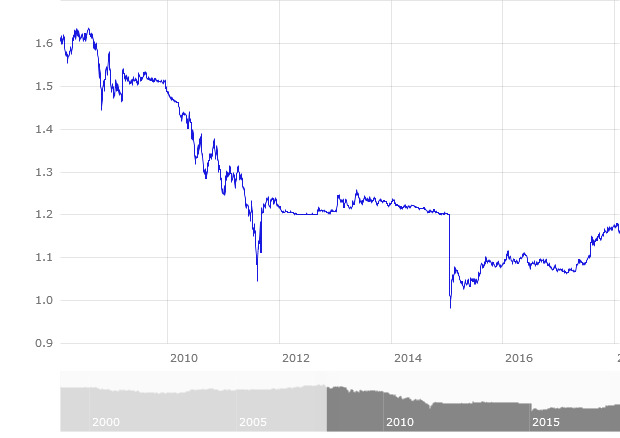
\includegraphics[width=\textwidth]{ECBExchangeRateEURvsCHF_31-01-2008_01-02-2018.jpg}
	
\end{figure}

% FIGURES GDPPC SPECIFICATIONS
\begin{subfigures}
\begin{figure}
	\caption{Specification 1 (baseline): GDP per capita Switzerland and synthetic control}
	
	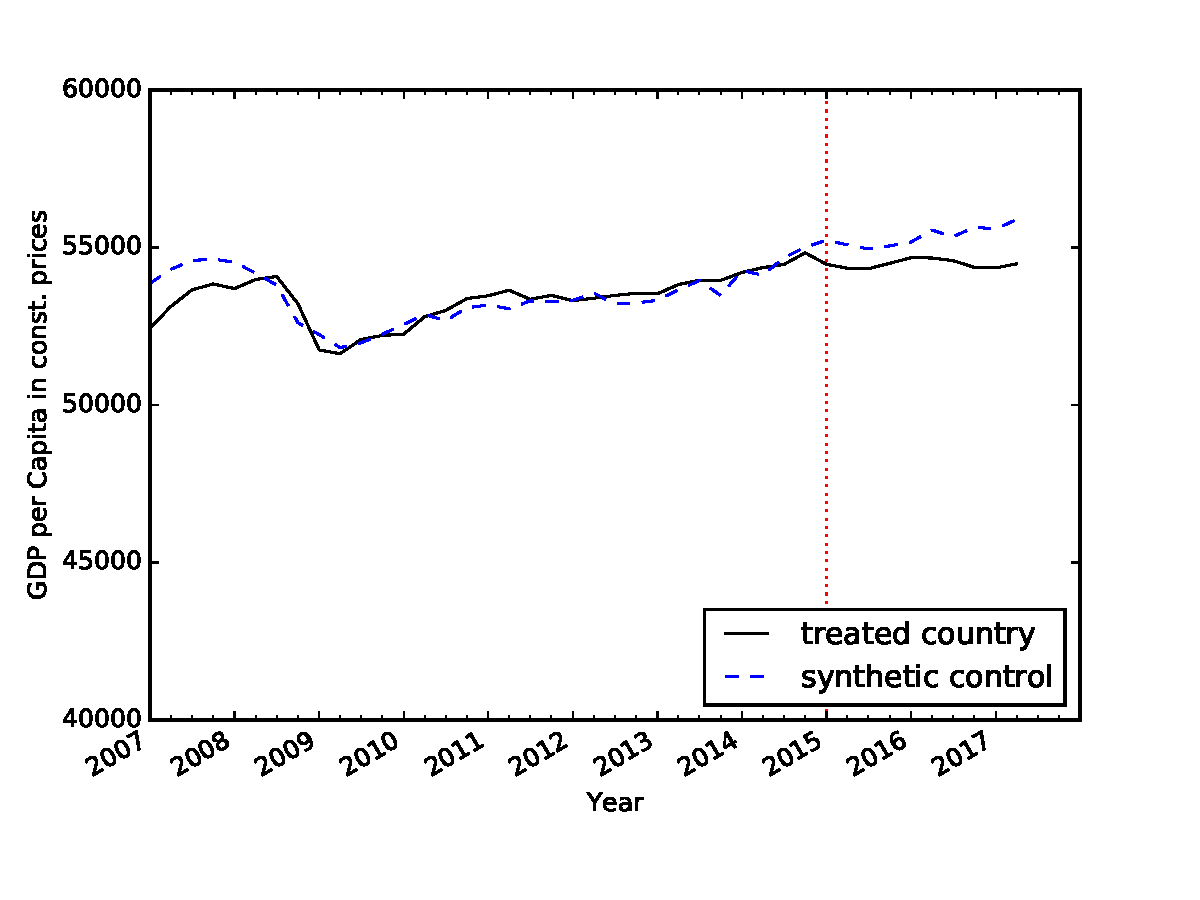
\includegraphics[width=\textwidth]{../../out/figures/sc_graph_gdppc_baseline.pdf}
	
\end{figure}

\begin{figure}
	\caption{Specification 2 (all year averages): GDP per capita Switzerland and synthetic control}
	
	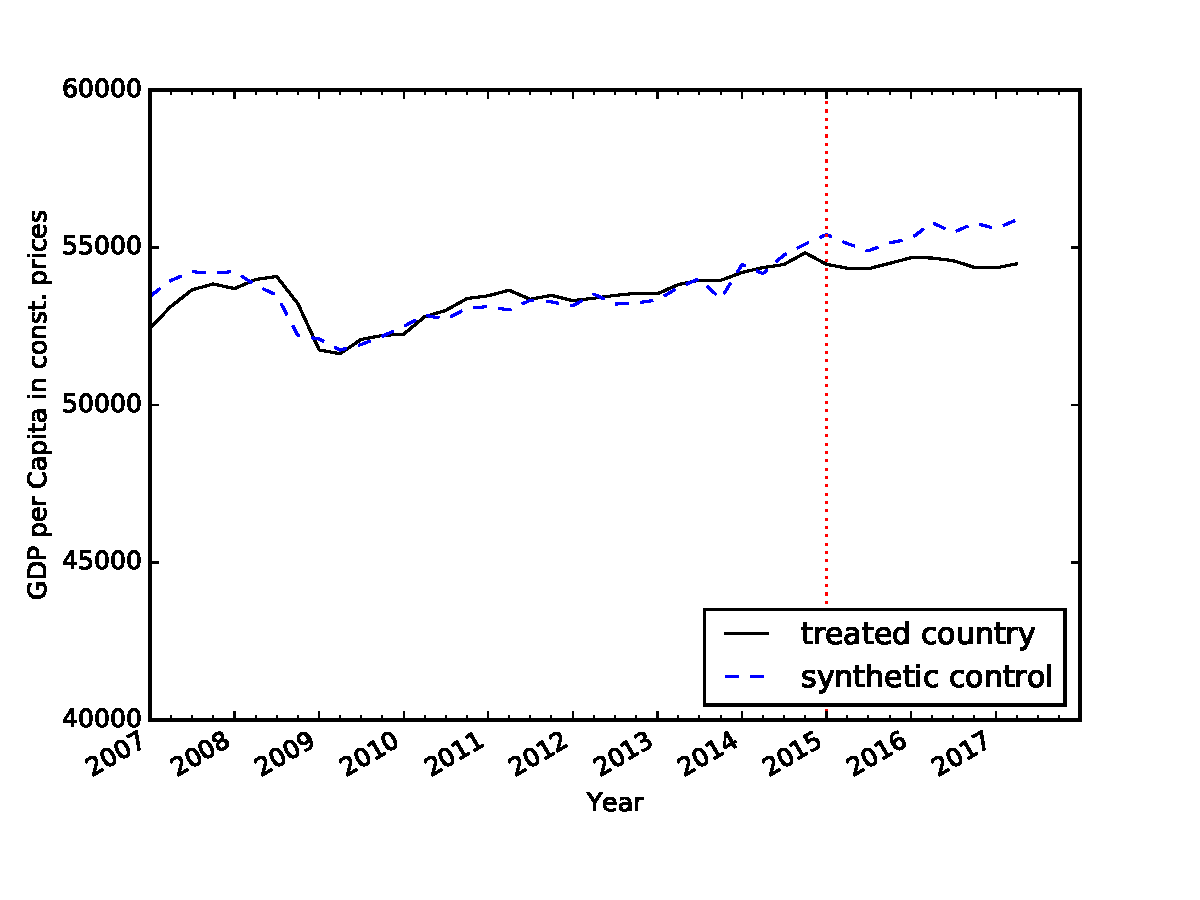
\includegraphics[width=\textwidth]{../../out/figures/sc_graph_gdppc_all_year_averages.pdf}
	
\end{figure}

\begin{figure}
	\caption{Specification 3 (including covariates): GDP per capita Switzerland and synthetic control}
	
	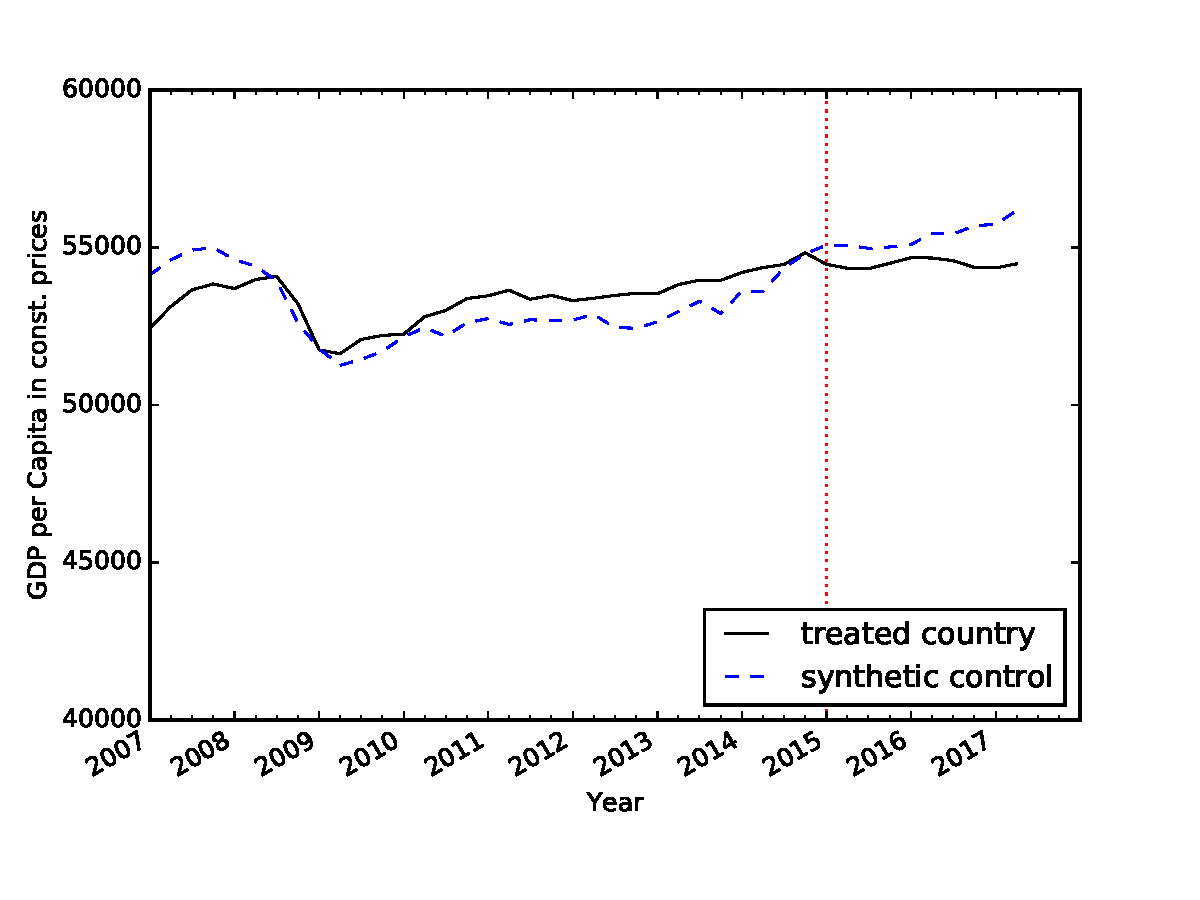
\includegraphics[width=\textwidth]{../../out/figures/sc_graph_gdppc_with_covariates.pdf}
	
\end{figure}
\end{subfigures}

% FIGURE CURRENT ACCOUNT
\begin{figure}
	\caption{Current account in \% of GDP Switzerland and synthetic control}
	
	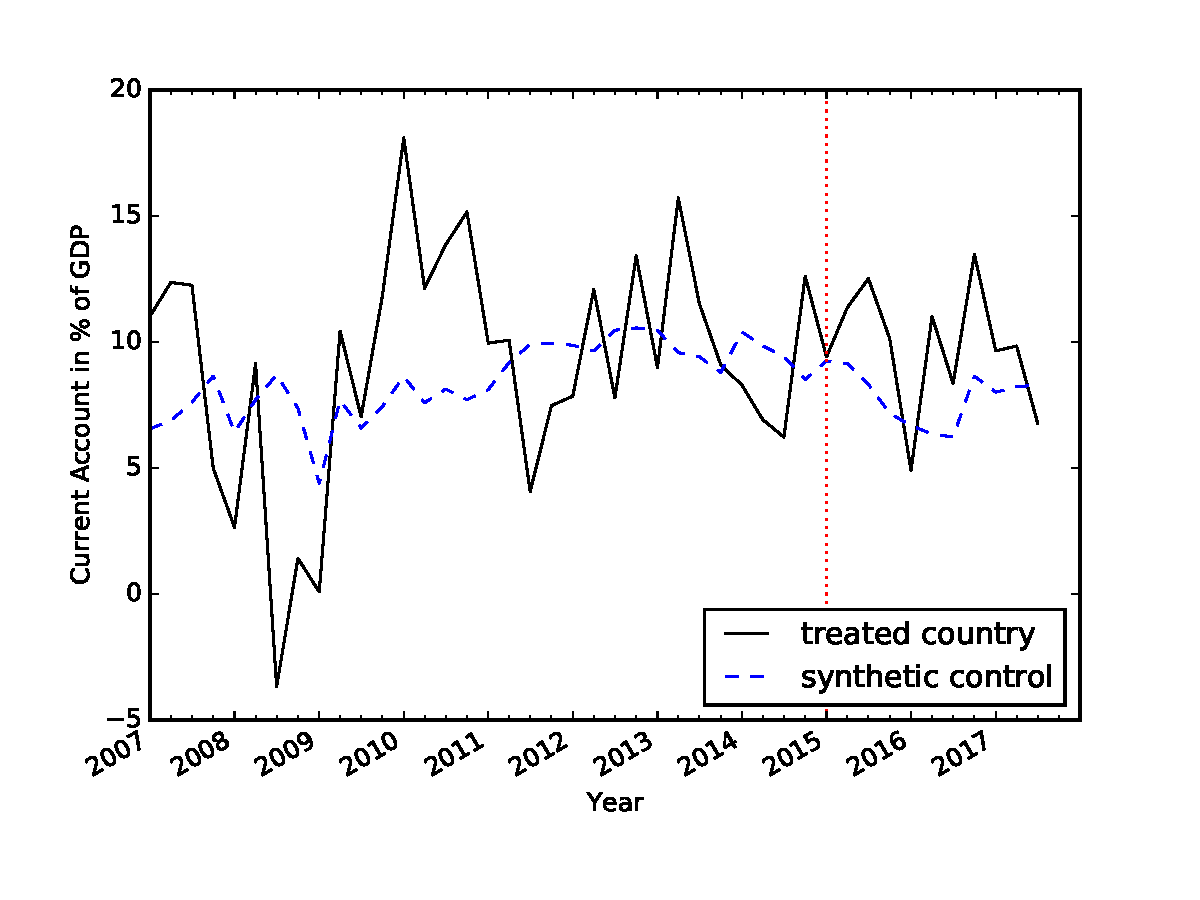
\includegraphics[width=\textwidth]{../../out/figures/sc_graph_ca_with_covariates.pdf}
	
\end{figure}

% FIGURES PLACEBO TESTS
\begin{subfigures}
	\begin{figure}
		\caption{Time Placebo (1997-2007Q2): GDP per capita Switzerland and synthetic control}
		
		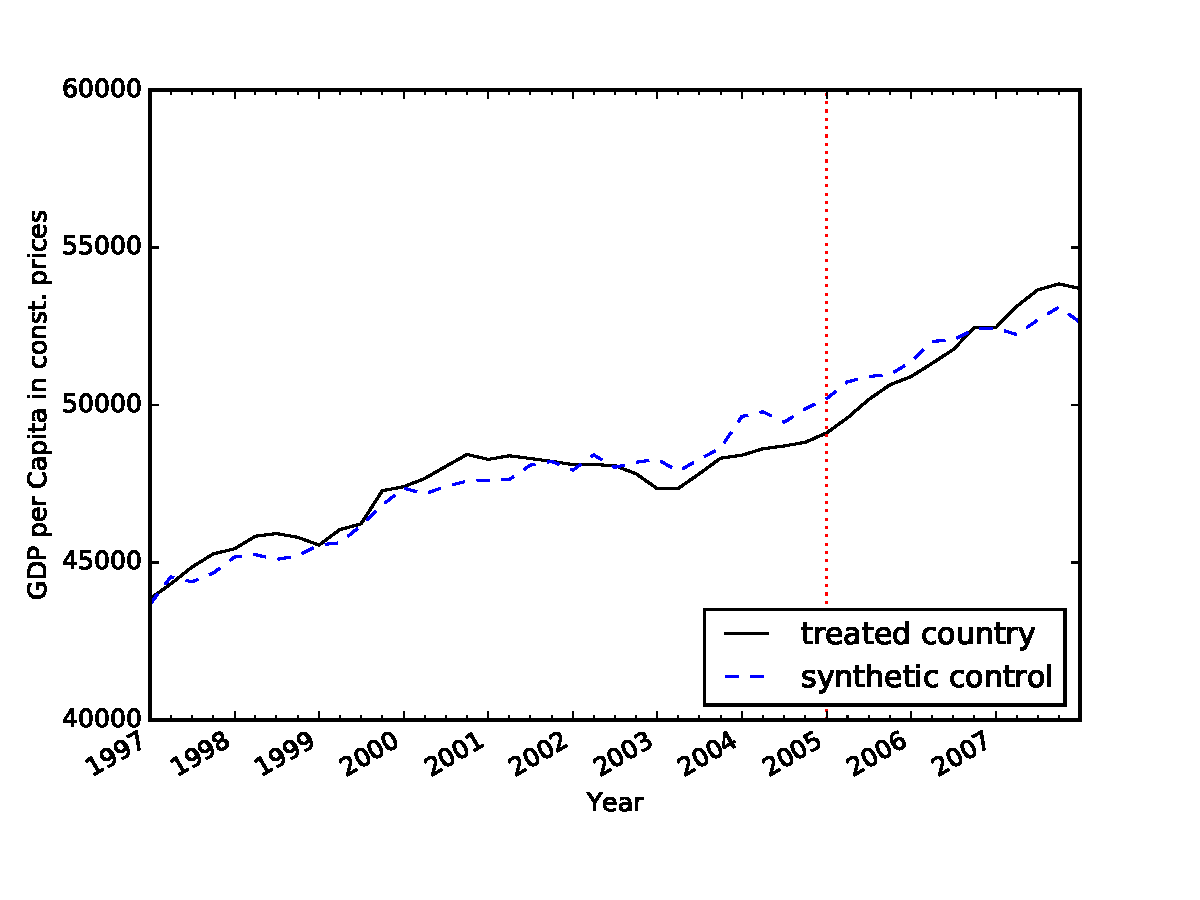
\includegraphics[width=\textwidth]{../../out/figures/sc_graph_gdppc_time_placebo.pdf}
		
	\end{figure}
	
	\begin{figure}
		\caption{Country Placebo: GDP per capita Australia and synthetic control}
		
		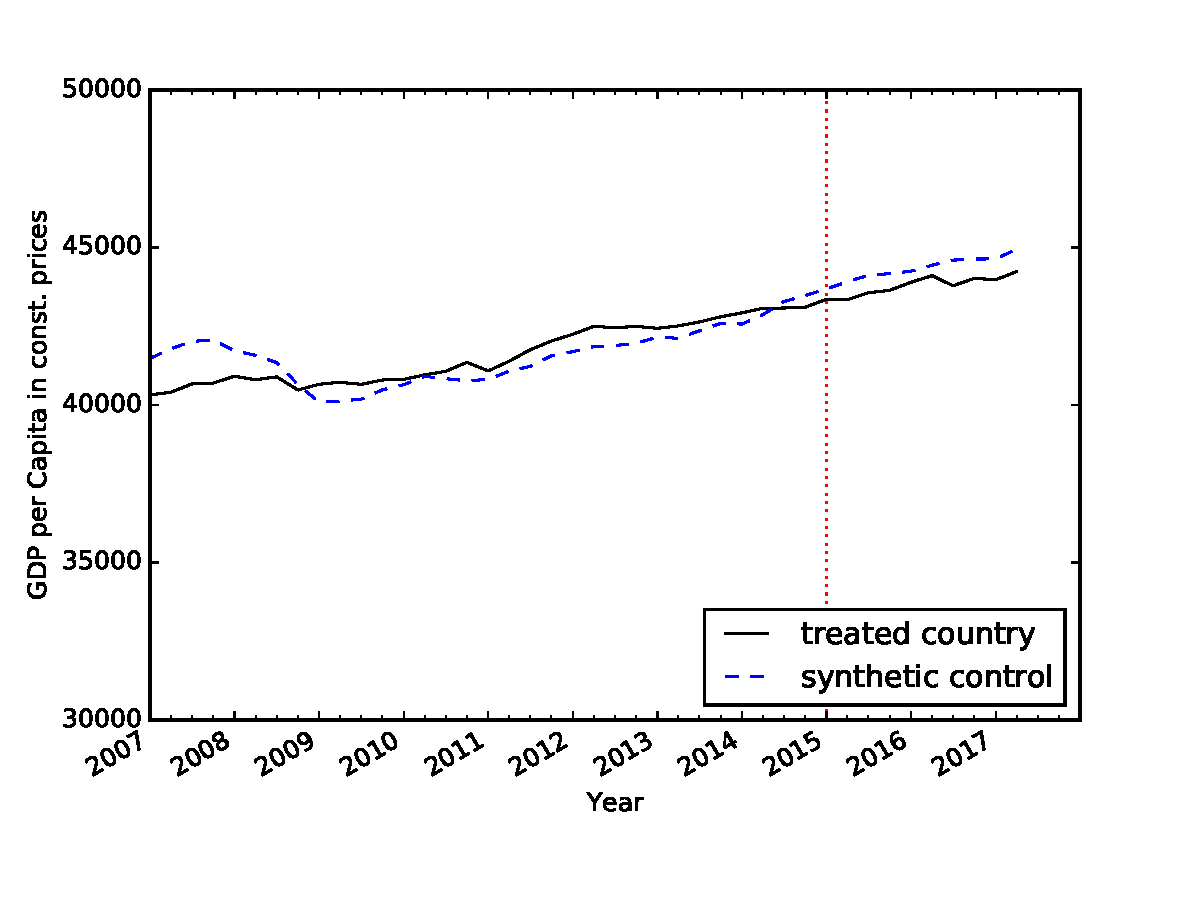
\includegraphics[width=\textwidth]{../../out/figures/sc_graph_gdppc_country_placebo.pdf}
		
	\end{figure}
	
\end{subfigures}



\clearpage


\setstretch{1}
\printbibliography
\setstretch{1.5}



\end{document}
